\documentclass[9pt,twocolumn,twoside]{osajnl}
\usepackage{comment}
\usepackage{threeparttable}
\usepackage{siunitx}
\usepackage{subcaption}
\usepackage{threeparttable}
\usepackage{siunitx}
\usepackage{multirow}
\usepackage{adjustbox}
\usepackage{ragged2e}
\setcounter{secnumdepth}{3}
\usepackage{stfloats}
\usepackage{afterpage}
\usepackage{graphicx}
\usepackage{float}
\usepackage{caption}
\usepackage{amsmath}
\usepackage{array}
\usepackage{lipsum}
% \usepackage{subfigure}
\usepackage[normalem]{ulem}
\journal{jocn} 
\newcommand{\red}[1]{\textcolor{red}{#1}}
\usepackage{afterpage}
\usepackage{makecell} % 在导言区添加这一行以引入宏包
\usepackage{tabularx} % 导言区加载 tabularx 宏包
\usepackage{cleveref}
\usepackage{xurl}
\Urlmuskip=0mu plus 1mu

% Set the article type for journal submissions. Comment out this line for Optica Open preprint submissions.
\setboolean{shortarticle}{false}
% true = letter / tutorial
% false = research / review article

\title{{Open-Source Cross-Domain Datasets Enabled by LLM-Driven Digital Twins and Network Telemetry}}

\author[1]{Sen Shen\textsuperscript{\textdagger,}}
\author[1]{Wanxin Zhao\textsuperscript{\textdagger,}}
\author[1]{Xuewen Chen\textsuperscript{\textdagger,}}

\author[1]{Jing Han}
\author[1]{Xueqing Zhou}
\author[1]{Ruizhi Yang}
\author[1]{Peiyun Ge}
\author[1]{Zhuojun Cai}
\author[1]{Vaigai Yokar}
\author[1]{Yulei Wu}
\author[1]{Shuangyi Yan*}
\author[1]{Dimitra Simeonidou}


\affil[1]{Smart Internet Lab, Faculty of Science and Engineering, University of Bristol, Bristol, United Kingdom.\newline
\textsuperscript{$\dagger$}These authors contributed equally to this work.}

\affil[*]{shuangyi.yan@bristol.ac.uk}




%% The publisher will insert the publication dates. The class supplies a
%% compilation date by default, so it must be explicitly cleared for review.
\dates{}

%% To be edited by editor
% The publisher will insert the final DOI after acceptance.  The class supplies
% a template DOI by default, so it must be explicitly cleared for submission.
\doi{}

\begin{abstract}

With the wide application of machine learning (ML) in telecommunication networks, networks are becoming increasingly intelligent and autonomous. However, sufficient practical data and high-quality synthetic data remain difficult to obtain for ML model training and updating. This challenge is more pronounced in cross-domain optical and wireless networks, where heterogeneous infrastructures, diverse telemetry interfaces, inconsistent data formats, and privacy concerns make data collection, alignment, fusion, and sharing particularly difficult. Meanwhile, generating high-quality synthetic data requires substantial human effort to design, configure, and validate diverse simulation scenarios. In this paper, we present an openly available cross-domain dataset framework combining network telemetry and semantic abstraction for practical data with a large language model (LLM)-driven multi-agent digital-twin (DT) workflow for generated data. Building on our optical telemetry platform, the framework integrates distributed and centralised data repositories, Kafka-based telemetry pipelines, DTs, AI engines, and network controllers to facilitate practical data collection, cross-domain fusion, and automated dataset generation. We release practical datasets from optical and wireless testbeds covering transmission performance monitoring, fibre sensing, and multi-access wireless network performance. Collected in different periods because of platform scheduling, these datasets enter the same training workflow through a unified data interface. We design and evaluate wireless semantic modules that transform raw telemetry into compact task-relevant representations, assessing task utility and observed attribute leakage. We also demonstrate an LLM-driven multi-agent DT workflow that translates high-level requests into executable scenarios, invokes optical and wireless simulators, analyses results, and supports refinement. Its optical configuration set is checked against deterministic enumeration and versioned GNPy replay.


\end{abstract}

\setboolean{displaycopyright}{false} % Do not include copyright or licensing information in submission.

\begin{document}

\maketitle

\section{Introduction}

In recent years, machine learning (ML) has been widely investigated in telecommunication networks to support intelligent and autonomous network operation. In optical networks, ML has been applied to quality of transmission (QoT) estimation, traffic prediction, anomaly detection, and resource allocation~\cite{villa2023IEEEAccess}. In wireless networks, ML-based methods have also been explored for radio resource management, multi-access optimisation, traffic prediction, mobility management, and service quality assurance~\cite{sun2019IEEE}. These advances indicate a clear trend towards AI-native network intelligence, where data-driven models support monitoring, optimisation, and closed-loop control.

However, the effectiveness of ML models strongly depends on representative data. Operational network records can expose topology, device configurations, traffic, and service conditions, which limits public release. Existing optical and wireless datasets~\cite{zhai2024alibaba,filer2016microsoft} also tend to address one domain, task, or experimental scenario. This restricts their applicability to converged optical and wireless networks, where heterogeneous infrastructures, telemetry interfaces, data formats, time scales, and privacy requirements complicate data collection, fusion, and reuse. Synthetic data can complement practical measurements by covering controllable or rare conditions, although DT-based generation still requires substantial effort to specify scenarios, execute simulations, and validate the results.

To address these challenges, we present an openly available dataset framework for optical transport, fibre sensing, and wireless access. The framework organises practical telemetry with common metadata and data-access conventions, and evaluates compact wireless semantic representations in a constructed optical--wireless learning benchmark. An LLM-driven multi-agent DT workflow generates complementary optical and wireless simulation records from configurable scenarios.

The main contributions are as follows. (1) We consolidate practical optical-transport, fibre-sensing, and multi-access wireless datasets with their acquisition context, formats, sampling information, provenance, and repository access terms. The telemetry platform builds on our previous implementations~\cite{shen2025telemetry,Shen2026OFCdata}; the present contribution is their dataset-level organisation and cross-domain interface. (2) We specify and evaluate hand-crafted and learned wireless semantic representations for optical--wireless fusion using chronological partitions, train-only preprocessing, repeated runs, conventional baselines, and multiple privacy attackers. (3) We demonstrate an LLM-driven multi-agent interface to GNPy and ns-3 DT engines and compare its optical configuration set with an independent deterministic enumerator. (4) We assess numerical reproducibility by rerunning 96 archived GNPy configurations in a v2.12-compatible environment and a schema-corrected v2.14.2 environment, quantifying output differences and identifying remaining physical-model calibration limitations.

The remaining sections are organised as follows. Section~II reviews cross-domain data availability and telemetry, semantic abstraction, DTs, and LLM-driven network automation. Section~III defines the framework scope, Section~IV describes the telemetry architecture, semantic-fusion benchmark, and practical datasets, Section~V presents the LLM-driven multi-agent DT demonstration, and Section~VI concludes the paper.

% \section{Related Work}
% \subsection{ML Applications}
% With the successful application of ML in natural language processing, ML techniques have been widely applied to optical and wireless networks over the past decade for performance prediction, resource allocation, and network optimisation. These advances have accelerated the evolution towards AI-native networks. More recently, LLMs with strong reasoning and task-planning capabilities, have further enhanced network automation and reduced human intervention.

% \subsubsection{Traditional ML in Optical and Wireless Networks}

% Traditional ML can be categorised into four distinct groups: supervised learning, unsupervised learning, and reinforcement learning. Supervised learning including Random Forest, Decision Tree, Support Vector Machine and neural networks, is widely used in QoT estimation and traffic prediction. For example, in optical networks, an RF-based ML equaliser was developed for DP-64QAM coherent optical transmission, achieving deep-learning-level equalisation performance with substantially lower computational complexity. Also, an SVM-based ML approach was introduced to estimate lightpath QoT in optical transport networks, achieving high classification accuracy and significantly reduced computation time compared with semi-analytical methods. And an ANN-based multi-channel QoT prediction framework was demonstrated using real field-trial monitoring and configuration data, showing that the ML-based method can achieve accurate Q-factor estimation for dynamic optical network optimisation. Similarly, an SVM-based secure wireless communication framework was introduced by constructing signal-derived features and artificial training data from wireless propagation signals to detect active eavesdropping at the physical layer. In wireless networks, artificial neural networks have been extensively used to learn complex relationships from network data and support intelligent functions such as prediction, classification, resource optimisation, and autonomous network management.

% Unsupervised learning such as K-means, autoencoder, DBSCAN, is widely used in tasks including anomaly detection and clustering. For example, A DBSCAN-based unsupervised anomaly detection loop was deployed in a microservice-based optical SDN controller, achieving scalable telemetry-driven monitoring without labeled training data and supporting up to 960 optical channels with 5–20 ms inference latency. Also, unsupervised DNN-based power control has been applied to energy-efficient wireless networks by directly optimising fractional energy-efficiency objectives through primal-dual learning, achieving real-time inference without requiring labeled solutions from conventional optimization algorithms. Compared with supervised and unsupervised learning, RL is mostly used in decision and control tasks. In optical networks, DRL is widely used in RMSA problem. For example, it has been applied to dynamic RMSCA in multi-core-fiber SDM-EONs, where PPO-based agents learn adaptive routing and core-allocation policies to improve spectrum utilization and reduce blocking probability under crosstalk constraints. In wireless networks, DRL is widely used to learn adaptive resource allocation and control policies under dynamic channel, traffic, and mobility conditions. In wireless networks, DRL is widely used to learn adaptive resource allocation and control policies under dynamic channel, traffic, and mobility conditions. For multi-server MEC networks, DRL has been used to support long-term resource planning, where DQN and multi-agent DDPG enable resource reservation and server cooperation, while optimization-based policies handle task offloading, transmission power allocation, and computing resource distribution.


% \subsubsection{LLMs in Networks}

% \subsection{Network Telemetry}


\section{Related Work}

\subsection{Cross-Domain Data Availability and Network Telemetry}
 
Representative data are essential for training, validating, and updating ML models in telecommunication networks. Optical-transport records may include bit error rate (BER), optical signal-to-noise ratio (OSNR), Q-factor, optical power, routes, equipment configurations, and alarms. Fibre-sensing datasets add state-of-polarisation (SOP) evolution, backscatter traces, distributed acoustic sensing signals, and vibration-related features~\cite{he2023isac,zhao2025vibration,zhao2026train}. Wireless-access telemetry commonly includes throughput, packet loss, delay, signal strength, cell load, mobility, traffic distribution, and per-device access statistics~\cite{3gpp28552,etsi128554}. These measurements support different tasks and are normally produced by domain-specific experimental or operational systems.


Operational data may expose network topology, configurations, device states, customer traffic, service conditions, and operator policies, thereby limiting public release. Available optical examples include the Microsoft wide-area backbone dataset~\cite{filer2016microsoft,delezoide2020field}, the Fraunhofer HHI QoT collections~\cite{bergk2022qotdataset}, and the Alibaba production-network dataset~\cite{zhai2024alibaba,he2023qot}. Other releases cover space-division-multiplexing networks, fibre sensing, optical-device modelling, and radio-over-fibre systems~\cite{akbari2025sdmdatasets,li2026dasdataset,yuan2026soadataset,zhao2026mmwavearof}. These resources are valuable within their stated scopes, but most remain limited to one domain, topology, task, or measurement campaign and use different formats and metadata.

Network telemetry provides systematic mechanisms for acquiring and storing such measurements~\cite{rfc9232}. Model-driven and streaming solutions based on NETCONF/YANG, gRPC, gNMI, and publish--subscribe mechanisms expose network states and performance data~\cite{rfc9232,gnmi2018}. Optical-network studies have demonstrated real-time monitoring, streaming-assisted diagnosis, Kafka-based data transfer, and platforms integrating time-series and configuration storage~\cite{paolucci2018telemetry,tanaka2021diagnosis,sgambelluri2022kafka,shen2025telemetry}; O-RAN and AI-native RAN architectures similarly expose radio and service context to AI/ML applications~\cite{mahmoud2026oranintelligence}. Most implementations nevertheless remain tied to a particular domain, interface, or monitoring task, and published datasets often lack a common description of their acquisition scope and provenance.

Building on our earlier telemetry implementations~\cite{shen2025telemetry,Shen2026OFCdata}, the present work advances beyond those domain-specific systems by placing optical-transport, fibre-sensing, and wireless-access sources within an implemented cross-domain architecture with common publication metadata and a unified training interface. The practical campaigns retain their original timestamps and cover different periods because the experimental platforms were scheduled separately. During downstream training, the unified interface invokes the appropriate domain-specific preprocessing and exposes optical and wireless features through the same model call. The following subsection examines how wireless telemetry can be represented compactly for cross-domain data sharing and fusion.

\subsection{Semantic Data Abstraction for Privacy-Aware Cross-Domain Fusion}

Cross-domain data fusion requires deciding which telemetry should be shared and retained. Directly exporting raw wireless records may introduce unnecessary communication and storage overhead while exposing device-specific or service-sensitive information. In multi-access wireless networks, such records may reveal device identity, access behaviour, traffic patterns, mobility states, and service conditions~\cite{8792139}. Compact task-relevant representations can reduce the exposed raw detail while retaining information needed by a specified downstream task.

Task-oriented semantic communication provides a principle for this abstraction by transmitting information relevant to downstream tasks rather than reconstructing every source observation with equal fidelity~\cite{xie2022task,ma2023explainable}. Expert-designed indicators and learned information-bottleneck encoders can summarise wireless load, link stability, access diversity, and congestion risk~\cite{alemi2017vib}. Compactness alone does not establish privacy, because sensitive attributes may remain inferable from the representation. Noise injection, adversarial objectives, and representation regularisation have therefore been studied to balance task utility against observed information leakage~\cite{alemi2017vib,edwards2016censor,madras2018fair,wang2024privacysemantic}.

Existing semantic-communication and privacy-aware representation studies mainly evaluate transmission efficiency or downstream accuracy within a single application setting. Fewer studies jointly report task utility, representation size, and attribute-inference attacks when the representation is exported for reuse. The present work therefore compares hand-crafted and learned wireless semantic modules under a common temporal protocol and evaluates their outputs in an optical--wireless semantic-fusion task.

\subsection{Digital Twins and LLM-Driven Data Generation}

The preceding subsections concern the collection and selective sharing of practical telemetry. Synthetic data expand this coverage to topologies, loading conditions, device settings, and rare failures that are difficult to observe in testbeds, while providing labels under controllable conditions. Network DTs provide a natural execution tool because they emulate network behaviour under configurable topology, traffic, device, channel, and service conditions~\cite{zhuge2023dt}.

In optical networks, GNPy provides an open and vendor-independent physical-layer modelling framework for emulating optical paths under configurable topology, equipment, channel loading, and transmission-parameter settings~\cite{curri2022gnpy}. Recent studies have used GNPy-based DTs to generate optical-network datasets under normal and degraded conditions, such as amplifier degradation, span-loss variation, and component misconfiguration~\cite{mohamed2025dtfailuredb,mohamed2025mlagentsdt}. In wireless networks, simulators and DT platforms, such as ns-3 and Colosseum, support repeatable packet-level, radio frequency, and protocol-stack emulation~\cite{riley2010ns3,polese2024colosseum}, while generative-AI-enabled wireless DTs have been explored for 6G modelling and scenario augmentation~\cite{tao2024wirelessdt,chai2024genaidt}. These studies demonstrate the value of DTs for controllable data generation. Nevertheless, DT-based dataset generation still requires substantial manual effort to define objectives, configure scenarios, execute simulations, validate results, and refine parameter settings. This process becomes costly when one study spans multiple simulator ecosystems with different abstractions, interfaces, and configuration formats.

Recent studies have begun to integrate LLMs, AI agents, and DTs to reduce the manual burden of network automation. In optical-network DT research, modelling, telemetry, self-learning, and lifecycle management have been identified as key components for intelligent optical networks~\cite{wang2024dtreview}. GPT-enabled DT assistants have also been demonstrated to interpret user intentions and interact with DT functions for autonomous optical-network management~\cite{zhang2024gptdtassistant}. In addition, DTs have been used to provide updated network states and pre-verify LLM-generated strategies before deployment, with demonstrations covering performance optimisation, protection switching, and recovery after fibre cuts~\cite{song2025llmdt}. Other studies have explored fine-tuned local agents, DT-aided wavelength-loading control, AI-agent integration, and field-trial demonstrations for optical-network lifecycle automation~\cite{sun2025localaiagents,liu2024autodtwave,zhuge2025dtaiagent,liu2026fieldtrial}. These studies demonstrate the potential of LLMs and AI agents to interact with DTs, but their focus remains on network operation and management rather than autonomous dataset generation.

The cited DT assistants and AI-agent studies automate parts of modelling and network operation, but they still rely on explicitly supplied objectives and configuration ranges~\cite{zhang2024gptdtassistant,song2025llmdt,sun2025localaiagents,liu2024autodtwave}. This leaves dataset generation as a distinct workflow-design problem. The present work therefore studies an LLM-driven interface that translates a high-level request into structured tasks, invokes optical and wireless DT engines, analyses generated KPIs, and proposes refinements. Section~\ref{sec:LLM} evaluates the workflow through an instrumented run, a deterministic configuration-set reference, and simulator replay tests.








\begin{figure*}[t]
    \centering
    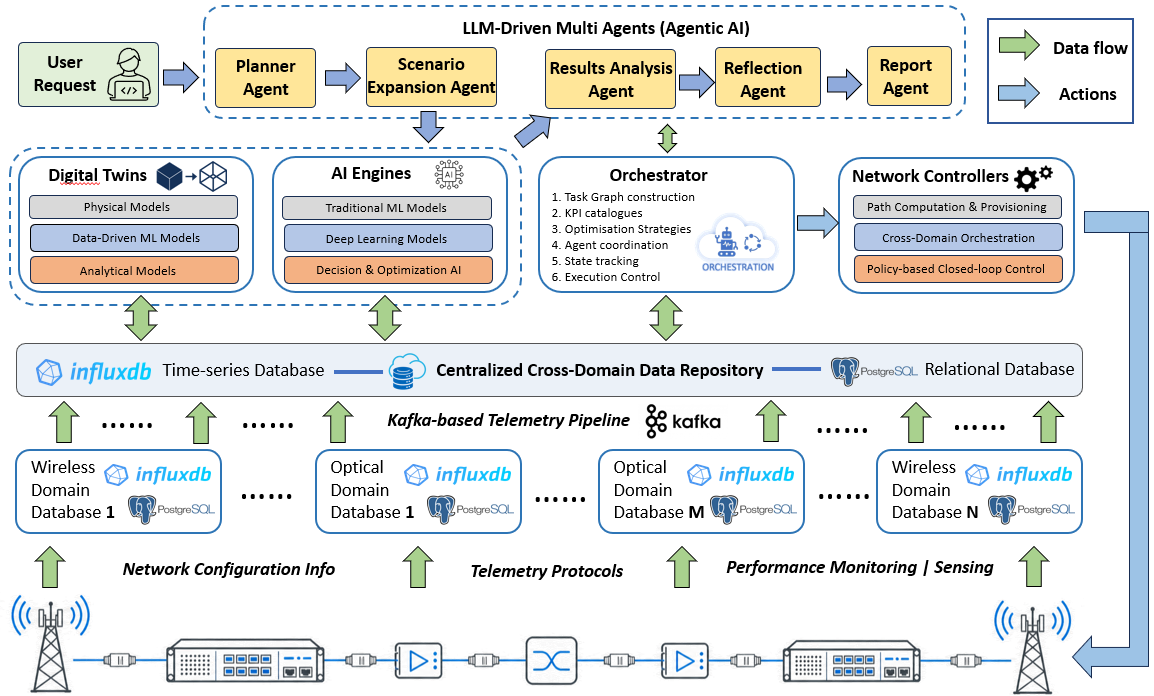
\includegraphics[width=0.95\linewidth]{Figures/architecture_v1.png}
    \captionsetup{justification=centering}
    \vspace{-0.1cm}
    \caption{System architecture for practical-data collection and DT-based dataset generation across optical and wireless domains. Green arrows indicate data exchange, and blue arrows indicate task or control actions.}
    \label{fig:proposed architecture.png}
    \vspace{-0.3cm}
\end{figure*}


\section{Unified Framework for Cross-Domain Dataset Collection and LLM-Driven Data Generation}

Figure~\ref{fig:proposed architecture.png} presents the layered architecture used to organise practical telemetry and generate complementary synthetic records across optical-transport, fibre-sensing, and wireless-access domains. At the physical-network layer, optical links interconnect wireless-access segments. Domain collectors export performance measurements, configuration records, and sensing data to distributed stores, while selected records are transferred to the central repository through the telemetry pipeline. Common metadata and data-access conventions allow these sources to be discovered and retrieved through one framework. The practical campaigns reported here cover different periods because of experimental-platform scheduling; the shared repository and interfaces provide cross-domain integration during data access and model training.

Two data workflows use this architecture. The practical-data workflow preserves the source records and their provenance, applies domain-specific preprocessing, and exposes optical and wireless features through a unified training interface. It also applies semantic abstraction to wireless telemetry before the constructed optical--wireless fusion task. The generated-data workflow translates a high-level request into structured tasks and simulator configurations, executes the corresponding GNPy or ns-3 DT, and retains the inputs, outputs, and execution logs. The two workflows therefore address complementary needs: practical measurements represent observed operating conditions, whereas DT-generated records extend coverage under configurable conditions.

Within the generated-data workflow, the orchestrator maintains the task state and schedules planning, scenario expansion, DT execution, result analysis, optional reflection, and reporting. It exchanges structured task descriptions and results with the functional roles in the Agentic AI layer and invokes the DT engines through simulator adapters. The AI-engine and SDN-controller services are inherited from our implemented telemetry platform~\cite{shen2025telemetry}, where OpenFaaS-hosted ML models consumed repository data and returned predictions to the controller for optical-link reconfiguration. Figure~\ref{fig:architecture_LLM} focuses on the new orchestrated data-generation sequence, while Fig.~\ref{fig:proposed architecture.png} shows how that sequence connects to the existing telemetry, intelligence, and control services.

The acquisition and storage functions build on our earlier telemetry implementations~\cite{shen2025telemetry,Shen2026OFCdata}. The present work connects the released domain datasets through common publication metadata and a unified training interface, introduces and evaluates the wireless semantic modules used in the fusion benchmark, and implements the traceable LLM-driven workflow for optical and wireless simulation. Section~\ref{sec:cross-domain-telemetry} describes the telemetry, repository, and semantic-processing functions, and Section~\ref{sec:LLM} details the orchestrated data-generation sequence and its evaluation.

\section{Cross-Domain Telemetry Architecture Across Optical and Wireless Networks}
\label{sec:cross-domain-telemetry}

\subsection{Proposed Cross-Domain Telemetry Architecture}
\label{subsec:4.A}

Figure~\ref{fig:cross-domain telemetry.png} presents the cross-domain extension of our implemented telemetry platform~\cite{shen2025telemetry}. The platform provides device-data acquisition, time-series and configuration storage, Kafka transfer, OpenFaaS-based AI services, and SDN-controller interfaces. This work adds wireless telemetry, exported-record semantic processing, the unified optical--wireless training interface, and the DT data-generation workflow described in Section~\ref{sec:LLM}.

\subsubsection{Optical Transport Network Physical Layer}

At the bottom of Fig. \ref{fig:cross-domain telemetry.png}, the physical layer of the optical transport network consists of multiple interconnected optical nodes, including aggregation and intermediate nodes. These nodes represent practical optical transport infrastructure, in which network elements such as transponders, fibre links, optical switches, reconfigurable optical add-drop multiplexers (ROADMs), and optical amplifiers generate heterogeneous operational data.

The collected optical domain data can be categorised into three types: performance monitoring metrics, equipment parameters and topology information, and fibre sensing data. Performance monitoring metrics include receiver-side BER, OSNR, received optical power, amplifier input/output power levels, and per-port optical power measurements from optical switches. Equipment parameters and topology information include transmitter-side launch power, wavelength allocation, modulation format, amplifier gain, node configuration, and link information. Fibre sensing data include SOP, chromatic dispersion (CD), polarisation mode dispersion (PMD), and backscatter traces. These data provide communication- and physical-layer visibility, supporting applications such as QoT estimation, anomaly detection, environment-aware operation, and proactive maintenance.

% These data provide visibility at both the communication and physical layers. Performance monitoring metrics support ML applications such as QoT estimation, whereas fibre sensing data enable environment-aware network operation, anomaly detection, and proactive maintenance.


\begin{figure*}[t]
    \centering
    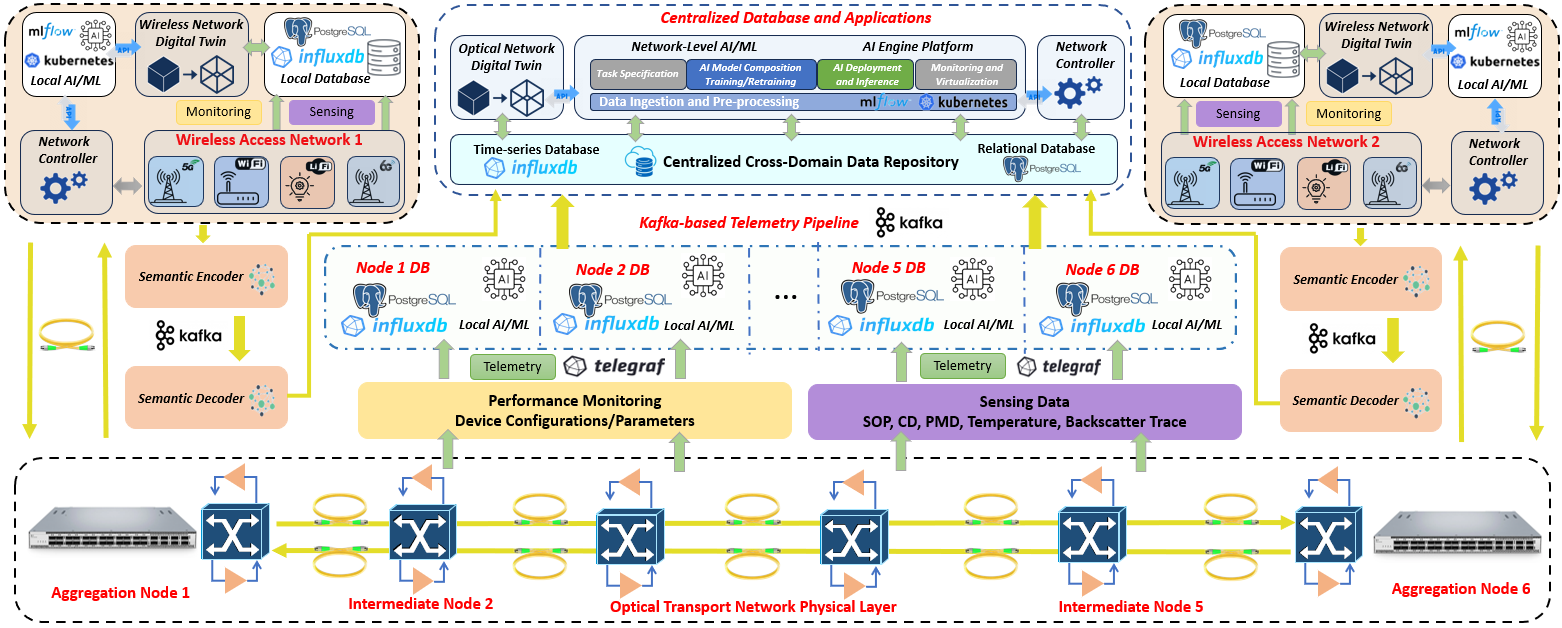
\includegraphics[width=\linewidth]{Figures/cross-domain telemetry.png}
    \captionsetup{justification=centering}
    \vspace{-0.1cm}
    \caption{Telemetry, repository, network-intelligence, and control services in the cross-domain framework. The optical telemetry, AI-engine, and SDN-controller implementation builds on the field-trial platform in~\cite{shen2025telemetry}; this work extends the data path to wireless telemetry, semantic processing, and DT-based data generation.}
    \label{fig:cross-domain telemetry.png}
    \vspace{-0.3cm}
\end{figure*}


\subsubsection{Distributed Node-Level Databases}
In the implemented optical telemetry platform, node-level databases retain measurements and the device context needed to interpret them. InfluxDB stores repeated, timestamped measurements such as BER, OSNR, optical power, and sensing streams; PostgreSQL stores structured records such as node and link topology, equipment settings, and configurations. This division keeps rapidly changing measurements associated with the more stable network description at their source. The central repository receives selected records from these local stores, while the practical wireless campaign supplies separately acquired testbed records to the unified data interface described in Section~\ref{subsec:SemanticModules}.

\subsubsection{Telemetry Service Design}

The telemetry service ingests monitoring and configuration records through the interfaces available on each device, including NETCONF, gRPC/gNMI, REST/HTTP, and vendor APIs. Telegraf acts as a metrics collection agent, while source-specific collectors handle other device outputs; the resulting measurements are written with timestamps to the local stores. Acquisition can therefore vary by source while retaining the timestamps and context needed for subsequent use.


For repository transfer, local services publish selected records to Kafka topics, which group records by stream. A central consumer subscribes to the relevant topics and writes the received records to the repository. This producer--consumer path connects the node-level stores to the shared data layer.

For the optical--wireless fusion benchmark, the evaluated semantic modules transform exported wireless records into compact task-related representations before they enter the shared training interface. Their design and evaluation are detailed in Section~\ref{subsec:SemanticModules}.

\subsubsection{Centralised Cross-Domain Data Repository}

The central repository provides a common access point for selected monitoring streams and their topology, equipment, and service context. It retains the storage distinction introduced above: time-series records remain associated with their source timestamps, while structured metadata identify the network elements and configurations to which they refer. The unified training interface then invokes domain-specific preprocessing and constructs task-specific optical--wireless feature records. As the practical campaigns occurred in different periods, the benchmark pairs their records by the explicit rule in Section~\ref{subsec:SemanticModules}.

\subsubsection{Network Intelligence and Controllers}

The AI engine and SDN controller were implemented and experimentally demonstrated with the optical telemetry platform in~\cite{shen2025telemetry}. ML models were deployed as OpenFaaS functions and accessed through HTTP interfaces. The reported field trial measured less than 0.05~s from the time-series database to the AI engine and less than 0.3~s for multi-link ANN-based QoT inference. The controller used the prediction output to reconfigure Voyager transponders; modulation-format and launch-power changes took approximately 180~s and 5~s, respectively. These services remain part of the architecture in Figs.~\ref{fig:proposed architecture.png} and~\ref{fig:cross-domain telemetry.png}. In the present extension, the repository supplies practical and generated records through the unified interfaces, while the orchestrator manages the DT-based generation sequence evaluated in Section~\ref{sec:LLM}.

% The AI engine platform provides network-level AI/ML capabilities, including data ingestion and preprocessing, task specification, model composition, training or retraining, deployment and inference, monitoring, and virtualisation. Containerised execution environments, such as Kubernetes, and model-management tools, such as MLflow, can support scalable AI/ML lifecycle management. By leveraging both real telemetry data from the centralised repository and synthetic data generated by digital twins, AI engines can perform tasks such as QoT estimation, anomaly detection and traffic prediction.

\subsubsection{Wireless Access Network Domains}

The wireless access domains in Fig.~\ref{fig:cross-domain telemetry.png} place heterogeneous 5G, Wi-Fi, and LiFi networks at the edges of the optical transport architecture. Access points and multi-connected CPEs provide per-interface traffic observations alongside access-link measurements, making both traffic distribution across RATs and link conditions visible. This access-side view complements the optical performance and fibre-sensing streams with information about the conditions experienced by connected devices. The practical wireless records were collected from the 5G-CLARITY/REASON multi-access testbed, whose configuration and dataset are detailed in Section~IV-C.

\subsection{Semantic Modules for Cross-Domain Data Fusion}
\label{subsec:SemanticModules}

The semantic module converts wireless telemetry into compact representations. We compare V1, a hand-crafted representation; V2, a learned eight-dimensional latent representation; and V3, a learned three-dimensional bottleneck with optional training-time noise. We use \emph{privacy-aware} to denote the explicit evaluation of representation dimension, training-time noise, and attribute leakage; the experiments quantify empirical leakage without providing a formal privacy guarantee.

%Fig.\ref{fig:telemetry service design.png} details the novel design of both the local telemetry service from the physical layer of the optical network to distributed databases and the remote telemetry service from distributed databases to the centralized database in the aforementioned proposed unified platform. 

\subsubsection{Semantic Module Designs}

The input contains 12 features derived from 30-s wireless records: aggregate 5G, Wi-Fi, and LiFi traffic; total traffic; mean Wi-Fi and LiFi signal levels; mean Wi-Fi inactivity; a five-record rolling traffic fluctuation; three RAT-activity indicators; and a combined signal-quality score. RAT activity is defined relative to the 25th percentile of training traffic. All min--max and standard scalers are fitted on the training period only. Four task-oriented targets are then formed: load $L$, access diversity $D$, link stability $S$, and congestion risk $C$. With $q$ denoting combined signal quality, $f$ normalised traffic fluctuation, and $i$ normalised inactivity,
\begin{align}
D &= (a_{5G}+a_{WiFi}+a_{LiFi})/3,\\
S &= \left[0.5q+0.3(1-f)+0.2(1-i)\right]_{[0,1]},\\
C &= \sigma(2L+1.5i+f-1.5S-0.8D),
\end{align}
where $[\cdot]_{[0,1]}$ denotes clipping and $\sigma(\cdot)$ is the logistic function. These variables were selected to cover traffic intensity, temporal stability, multi-access availability, and a composite risk indicator using fields present across the wireless testbed exports. A confidence value $1-f$ accompanies each transmitted representation. Fig.~\ref{fig:semantic modules.png} summarises the three designs.

V1 transmits eight deterministic indicators: $L$, $S$, $D$, $C$, rolling-mean traffic, traffic fluctuation, signal quality, and inactivity risk. V2 uses a 12--64--32--8 encoder and a symmetric decoder to reconstruct $L$, $S$, $D$, and $C$. V3 uses a 12--32--16--3 encoder and a symmetric decoder. Its primary setting injects zero-mean Gaussian noise with $\sigma=0.05$ at the encoder input during training. The encoder--decoders use mini-batch Adam, batch size 32, at most 200 epochs, and early stopping with patience 12 on validation loss. For utility evaluation in the constructed benchmark, the four decoded targets plus confidence are concatenated with optical features; the privacy attacker receives the latent code plus confidence. The source, exact seeds, preprocessing parameters, and per-seed outputs are released with the experiment scripts.

\begin{figure}[h]
    \centering
    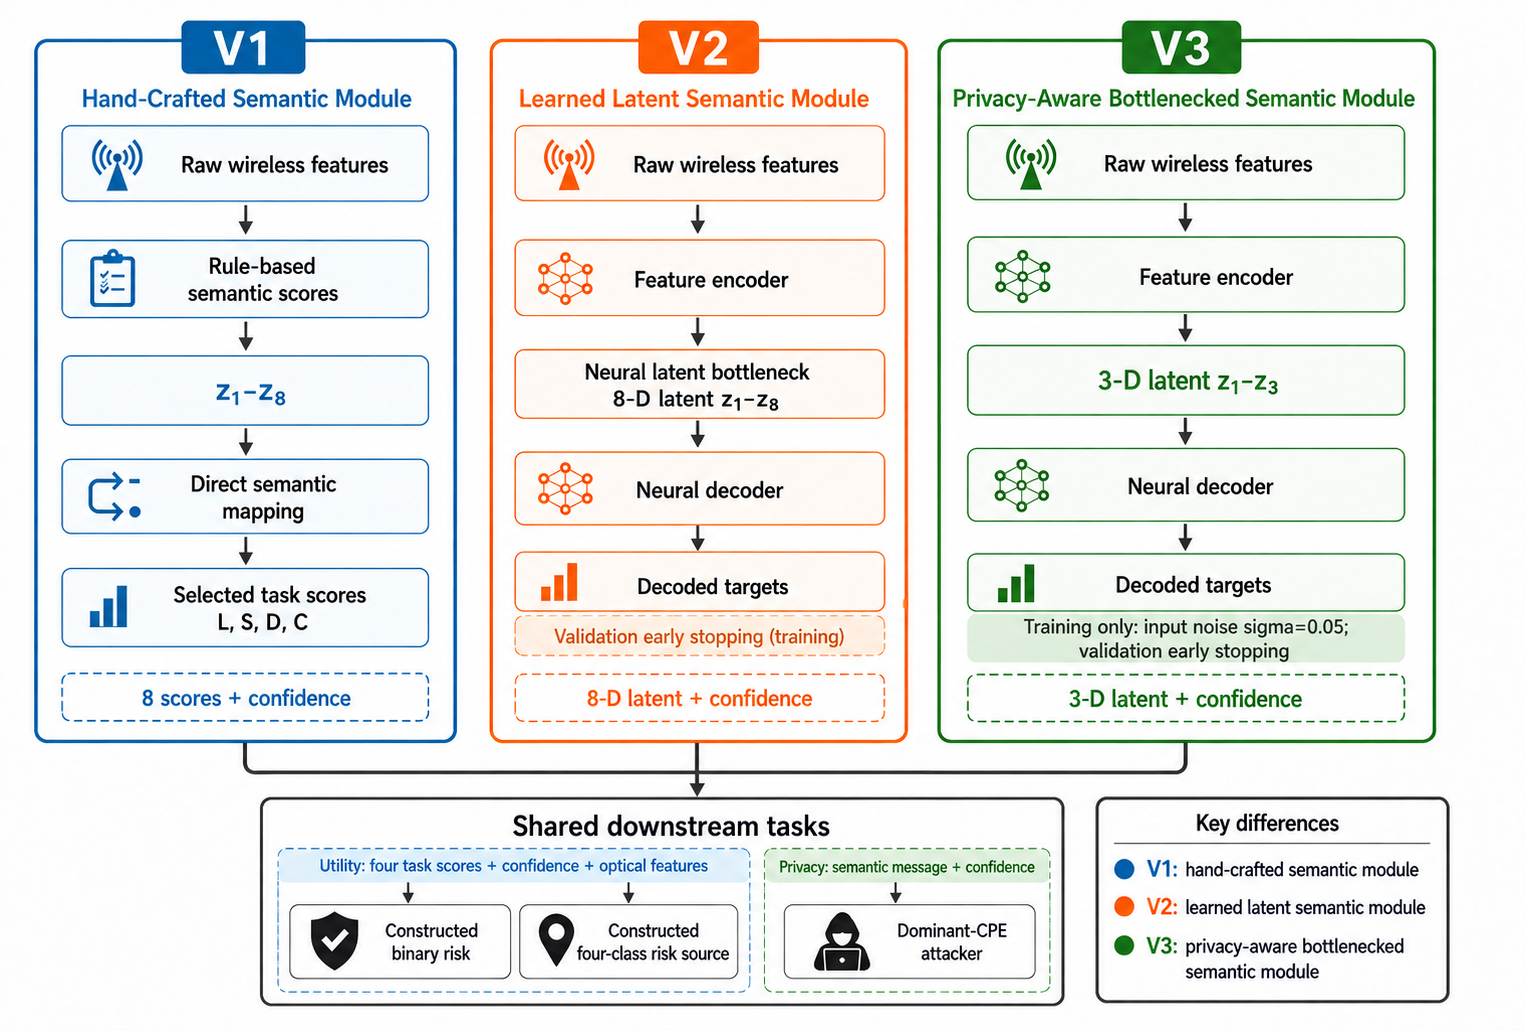
\includegraphics[width=\linewidth]{Figures/semantic_case_V1_V2_V3_principle_comparison_revised.png}
    \captionsetup{justification=centering}
    \caption{Three semantic-module designs and their evaluation inputs. Utility tasks use four task scores and confidence with optical features; CPE-attribute inference uses the semantic message and confidence.}
    \label{fig:semantic modules.png}
\end{figure}

The practical optical and wireless records were collected in different time periods because the experimental platforms could not be scheduled for concurrent acquisition. For subsequent training, a unified data interface loads both sources, invokes their domain-specific preprocessing functions, and returns a common feature record to the learning pipeline. The resulting fusion table maps the ordered 20,960 optical records to the ordered 2,849 wireless records at uniformly spaced relative positions. After one-step target shifting, 2,848 samples remain. Optical risk is defined using the training-period 15th percentile of Q-factor or 85th percentile of BER. Wireless risk is defined as $C>0.65$, $S<0.35$, or $D<0.34$. The binary label is their logical OR; four classes denote neither, wireless only, optical only, and both. These rule-derived labels provide reproducible benchmark risk conditions and do not represent observed service incidents.


\subsubsection{Testing Results}

Samples are partitioned chronologically into 60\% training, 20\% validation, and 20\% test segments, with a ten-record purge gap before each boundary to prevent five-record rolling features crossing partitions. This yields 1,698/560/570 evaluated samples. Every threshold, scaler, encoder, and downstream classifier is fitted after the split using training data only. Utility is measured with a 300-tree class-balanced random forest over ten seeds (3, 7, 11, 19, 23, 31, 42, 53, 71, and 97). We report Accuracy, Balanced Accuracy, Macro-F1, AUROC, and AUPRC; Table~\ref{tab:semantic_module_results} shows the primary Macro-F1 results and 95\% confidence intervals.

Privacy is operationalised as attribute inference from the transmitted representation. Dominant CPE and dominant RAT are defined by the largest aggregate traffic contribution in each record. Four attackers are evaluated: class-balanced logistic regression, a 300-tree random forest, a two-layer MLP (32 and 16 units), and histogram gradient boosting. Raw telemetry, PCA, random projection, majority, and stratified-random baselines are included. Because the test set contains 559 Wi-Fi and only 11 LiFi records (and no 5G record), RAT accuracy is dominated by the 0.981 majority baseline and is retained only as a diagnostic. CPE Macro-F1 is the primary privacy metric.

\begin{figure*}[t]
    \centering
    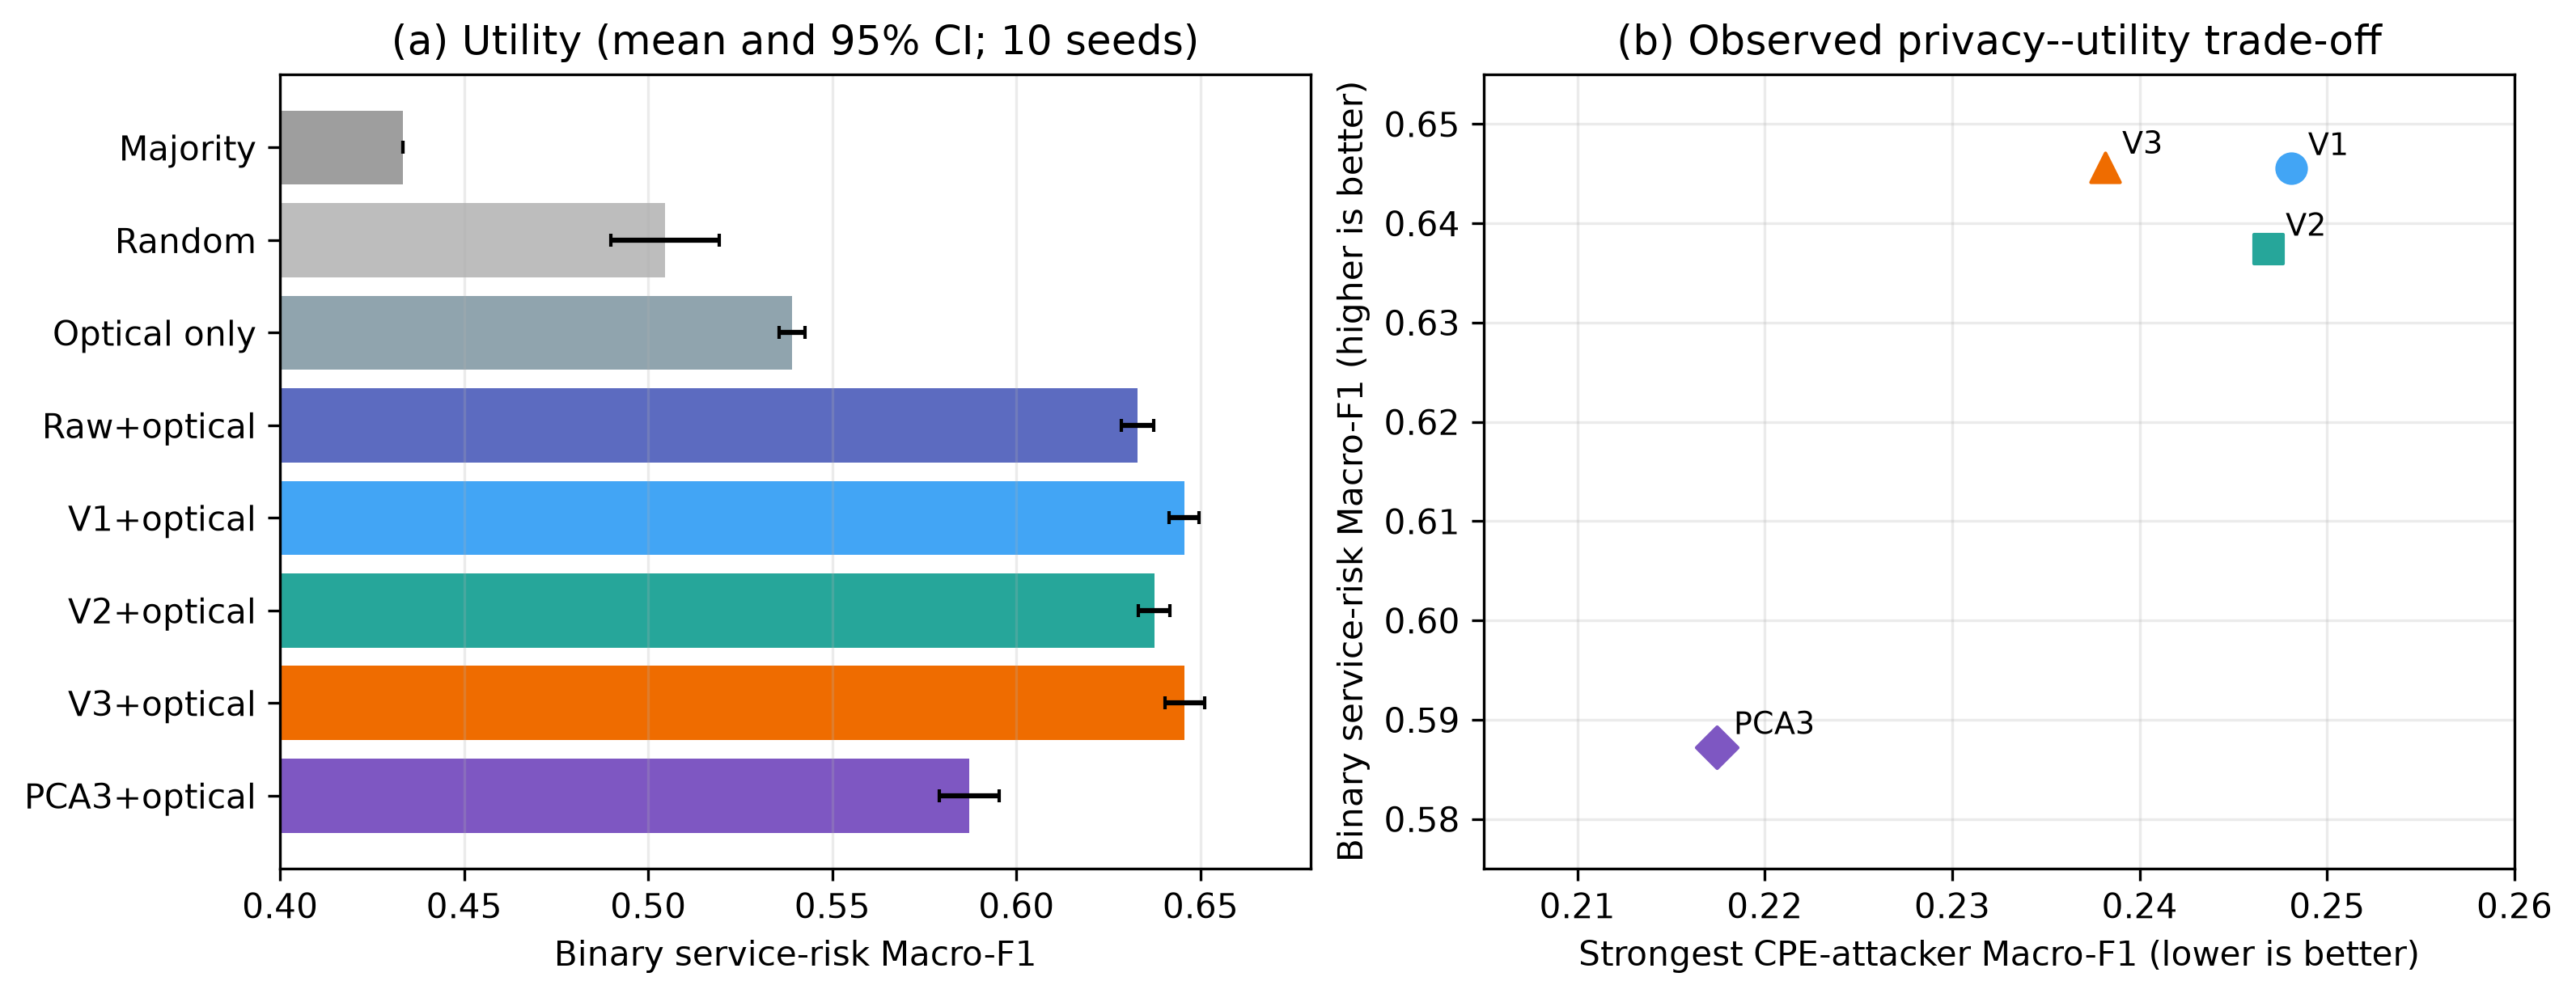
\includegraphics[width=0.98\linewidth]{Figures/semantic_module_revision_results.png}
    \captionsetup{justification=centering}
    \vspace{-0.1cm}
    \caption{Leakage-free temporal evaluation on the optical--wireless semantic-fusion benchmark. (a) Binary utility; error bars are 95\% confidence intervals over ten seeds. (b) Utility versus the strongest observed CPE attacker among four attacker families. Lower attacker Macro-F1 indicates less observed leakage but is not a formal privacy guarantee.}
    \label{fig:semantic results}
    \vspace{-0.2cm}
\end{figure*}

V3 reaches binary Macro-F1 $0.6457\pm0.0054$, similar to V1 ($0.6455\pm0.0040$) and above raw wireless plus optical features ($0.6329\pm0.0044$). The overlapping intervals indicate comparable V1 and V3 performance under this protocol. For the four-class task, raw features perform best. Moreover, the test distribution is 436/115/13/6, so the four-class result is exploratory. Removing V3 training noise slightly increases binary Macro-F1 from 0.6457 to 0.6473; increasing noise to $\sigma=0.10$ lowers the strongest CPE-attack Macro-F1 to 0.2319. Thus, noise reduces observed leakage but does not improve utility in this dataset.

\begin{table*}[t]
\caption{Temporal-holdout utility and CPE-attribute leakage (mean $\pm$ 95\% confidence interval over ten seeds).}
\label{tab:semantic_module_results}
\centering
\small
\setlength{\tabcolsep}{6pt}
\renewcommand{\arraystretch}{1.15}
\begin{tabular}{lccc}
\hline
Representation & Constructed binary Macro-F1 & Constructed four-class Macro-F1 & Strongest CPE-attack Macro-F1$\downarrow$ \\
\hline
Majority baseline & $0.4334\pm0$ & $0.2167\pm0$ & $0.1235\pm0$ \\
Stratified-random baseline & $0.5046\pm0.0147$ & $0.2427\pm0.0101$ & $0.2530\pm0.0095$ \\
Raw wireless + optical & $0.6329\pm0.0044$ & $\mathbf{0.4161\pm0.0051}$ & $0.2757\pm0$ \\
V1 + optical & $0.6455\pm0.0040$ & $0.3823\pm0.0033$ & $0.2481\pm0$ \\
V2 + optical & $0.6374\pm0.0044$ & $0.3958\pm0.0175$ & $0.2469\pm0.0102$ \\
V3 + optical ($\sigma=0.05$) & $0.6457\pm0.0054$ & $0.3955\pm0.0185$ & $0.2382\pm0.0113$ \\
PCA3 + optical & $0.5872\pm0.0081$ & $0.3829\pm0.0045$ & $\mathbf{0.2174\pm0.0059}$ \\
\hline
\end{tabular}
\end{table*}


Within the fusion benchmark, V3 offers a balanced operating point: it retains V1-level binary utility with moderately lower observed CPE leakage. PCA3 favours lower leakage at a larger utility cost, whereas raw features give the highest four-class utility. The term privacy-aware reflects this measured utility--leakage design objective.



\subsection{Practical Dataset Description}

The telemetry architecture organises optical-transport, fibre-sensing, and wireless-access datasets and their associated evaluation artefacts~\cite{Shen_dataset_2025}. Experimental-platform usage constraints required the practical campaigns to be conducted in different periods. The released files retain their source timestamps, and the training pipeline accesses them through the unified data interface described in Section~IV-B. Table~\ref{tab:dataset_summary} summarises each dataset's scope, contents, format, size, and reuse terms. Data and metadata distributed through the practical-data and revision repositories use Creative Commons Attribution--NonCommercial 4.0 International (CC BY-NC 4.0); cited external sources retain their own terms. A Croissant~1.0-compatible JSON-LD record provides file-level access locations, sizes, checksums, and source-defined units. The synthetic wireless data and source code are provided in the cited workflow repository~\cite{JOCN_revision_code_2026}.

\begin{table*}[t]
\caption{Summary of the practical, constructed, and synthetic datasets used in this paper.}
\label{tab:dataset_summary}
\centering
\scriptsize
\setlength{\tabcolsep}{3.5pt}
\renewcommand{\arraystretch}{1.05}
\begin{tabularx}{\textwidth}{p{2.4cm}p{3.0cm}X p{2.5cm}p{2.1cm}}
\hline
Dataset & Records/sampling & Principal fields or labels & Format/processed size & Access/reuse terms \\
\hline
339-km NDFF monitoring (2023--24) & 1,373 records; 10-s acquisition resampled to 15 min & Four Voyager BER channels, four derived Q-factors, timestamps & CSV + scripts; 0.15 MB & CC BY-NC 4.0 \\
339-km NDFF Voyager (2025--26) & 20,960 records; mostly 70--72-s spacing with gaps & Eight BER channels, timestamps, derived Q-factors & CSV; 1.79 MB & CC BY-NC 4.0 \\
986-km NDFF QoT & Two links and ROADM nodes; count unavailable & 12 channel states and Q-factors at three nodes & External CSV; size unavailable & Cited external source \\
Urban fibre sensing & Four weeks; 7.776- and 8-km links; 97.656~kSa/s polarimeter & BER, Q-factor, OSNR, power, $S_1$--$S_3$, time/voltage & MAT + CSV; size unavailable & Cited external source \\
Wireless access & 2,849 records over 24 h; nominal 30-s sampling; 46 fields & CPE traffic; 5G, Wi-Fi, and LiFi status/performance & CSV; 0.79 MB & CC BY-NC 4.0 \\
Synthetic GNPy optical DT & 8,192 executions; 6,144 unique configurations; 96 replays & Path, modulation/slot width, occupancy, power, GSNR, status, warnings & CSV + JSON/JSONL; 10.09 MB & CC BY-NC 4.0 \\
Synthetic ns-3 wireless DT & 48 configurations; 432 application flows; 624 raw FlowMonitor rows; 10-s runs & LTE/EPC, Wi-Fi 802.11n, and CSMA-based LiFi-surrogate settings; per-flow packet counts, throughput, delay, and jitter & CSV + XML/JSON/C++; 1.36 MB table & CC BY-NC 4.0 \\
Cross-domain semantic-fusion benchmark & 2,848 samples; chronological 1,698/560/570 split & Source indices, semantics, optical features, thresholds, binary/four-class labels & CSV; 1.60 MB & CC BY-NC 4.0 \\
\hline
\end{tabularx}
\vspace{2pt}
\footnotesize Sizes refer to principal processed files. File-level details and units are provided in the Croissant record and data dictionaries; unavailable values for cited external sources are left blank.
\end{table*}

\begin{figure*}[t]
    \centering
    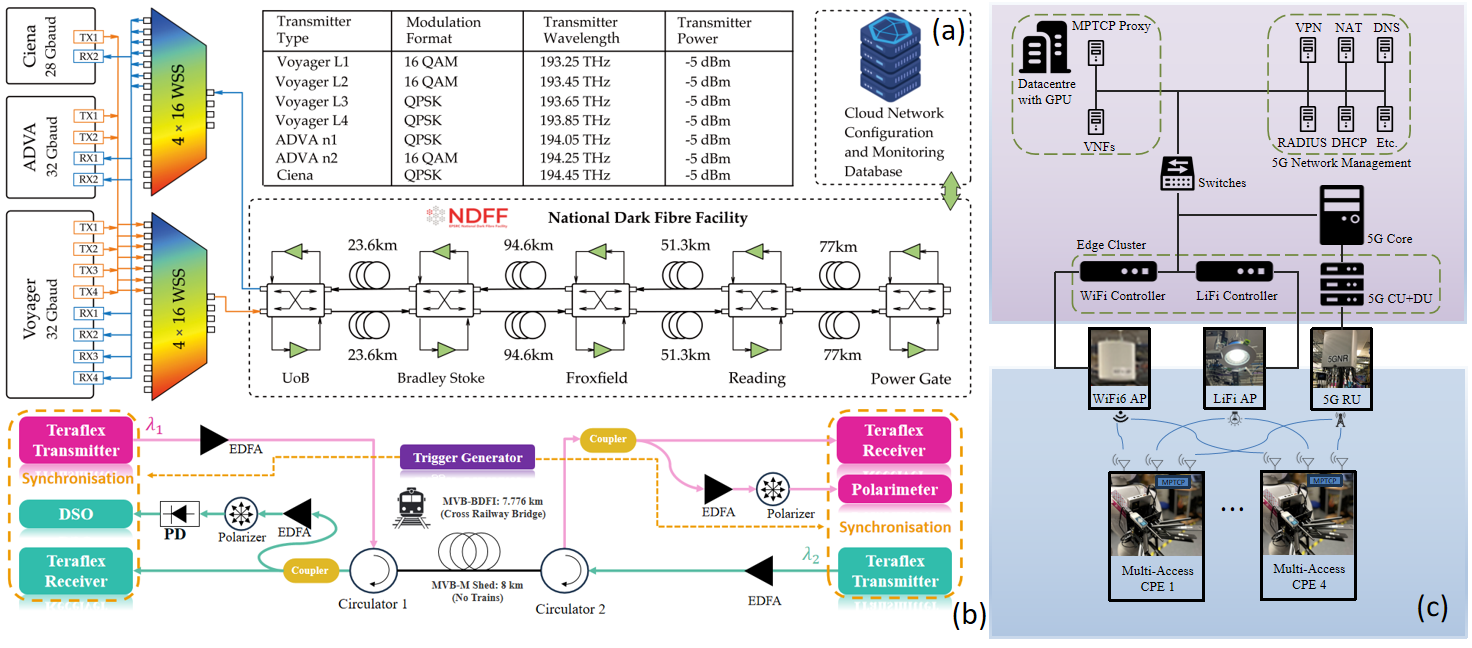
\includegraphics[width=\linewidth]{Figures/setup.png}
    \captionsetup{justification=centering}
    \vspace{-0.1cm}
    \caption{Experimental setups for practical dataset collection: (a) optical transmission performance monitoring over the NDFF, (b) bidirectional fibre sensing over deployed urban fibre links, and (c) multi-access wireless network testbed.}
    \label{fig:setup.png}
    \vspace{-0.3cm}
\end{figure*}

\subsubsection{One-Month Performance Monitoring Data from Optical Transport Network over NDFF}


Figure~\ref{fig:setup.png}(a) presents the experimental setup over part of the UK National Dark Fibre Facility (NDFF), including transponders, erbium-doped fibre amplifiers, wavelength-selective switches, and optical switches. Seven equalised 200-GHz-spaced PM-16QAM/QPSK signals were generated by Facebook Voyager, ADVA FSP~3000 TeraFlex, and Ciena transponders. Voyager and ADVA support 16QAM and QPSK, whereas the Ciena device supports QPSK. The signals traversed the 339-km loop from Bristol through Bradley Stoke, Froxfield, Reading, and Power Gate, with carrier frequencies from 193.25 to 194.45~THz. The launch power was fixed at $-5$~dBm for this measurement campaign. A cloud configuration and monitoring database stored the field-trial measurements.

The public repository distinguishes two measurement campaigns on this same 339-km loop. The earlier release contains 1,373 processed records collected from 26th December 2023 to 26th January 2024. Its 10-s raw BER measurements were resampled to 15-minute intervals, and four Voyager-channel Q-factors were calculated using $Q = \sqrt{2}\,erfcinv(2\,BER)$. This preprocessing reduces short-term measurement noise and aligns the sampling interval with that of the Microsoft open-source dataset.

A separate Christmas 2025 campaign, used as the optical source for the semantic-fusion benchmark in Section~IV-B, contains 20,960 valid eight-channel BER records from 22nd December 2025 16:38:43 to 24th January 2026 16:10:55. These are real acquisition timestamps retained without shifting or anonymisation. The raw CSV preserves 38 embedded headers from 39 concatenated acquisition segments; the released preprocessing removes those header rows before timestamp and BER parsing. Consecutive valid records are mostly 70--72~s apart, with larger acquisition gaps, and this file was not resampled to 15-minute intervals. Its unchanged source file and SHA-256 checksum are published with the acquisition note~\cite{Shen_dataset_2025}. Because the two campaigns differ in date, channel count, and sampling, they are reported as separate products rather than as stages of one transformation.

We also release a complementary dataset from a previous 986-km NDFF field trial~\cite{YangOFC2023} comprising two fibre links and ROADM nodes, where multi-channel Q-factor measurements were collected for end-to-end QoT prediction. Together, the 339-km and 986-km datasets provide representative short- and long-link field-trial scenarios for QoT estimation, short-term performance forecasting and anomaly detection.


\vspace{-0.2cm}
\subsubsection{Four-Week Sensing Data from BDFI and M Shed}

Figure~\ref{fig:setup.png} (b) illustrates the experimental setup for long-term fibre sensing based on bidirectional transmission. The experiment was conducted over two deployed urban fibre links in Bristol: a 7.776-km link connecting our lab in Merchant Ventures Building (MVB) to Bristol Digital Futures Institute (BDFI), and an 8-km link connecting MVB to M Shed Museum. Along the MVB-BDFI route, the fibre passes beneath multiple railway tracks near Bristol Temple Meads Station at the 3.2-km point, where it laterally traverses beneath a railway bridge. In contrast, the MVB-M Shed route does not pass beneath railway tracks.

An ADVA FSP 3000 Teraflex transponder generated two 32-GBaud PM-QPSK optical signals, which were launched into the fibre links through optical circulators to enable counter-propagating transmission. The endpoint circulators were interconnected through the live field fibre, with the forward and backward channels centred at 193.4 THz and 191.3 THz, respectively. At each endpoint, the received optical signal was split using an optical coupler: 90\% of the optical power was directed to the coherent receiver, while the remaining 10\% passed through a polariser and was delivered to a polarimeter and a real-time oscilloscope equipped with a photodetector. This configuration enables simultaneous communication monitoring and fibre sensing. The polariser projects the received state of polarisation (RSOP) onto a fixed eigenstate, allowing environmental disturbances along the fibre to be captured through the measured polarisation dynamics. For vibration localisation, a common trigger from an arbitrary waveform generator was used to synchronise both the polarimeter and oscilloscope.

The dataset spans four weeks and is provided in MAT and CSV formats. It contains communication KPIs, including BER, Q-factor, and OSNR, and polarisation telemetry (Stokes parameters $S_1$, $S_2$, and $S_3$). These measurements were continuously collected by the ISIC end-to-end monitoring platform. Because the data originate from deployed urban fibres rather than laboratory spools, they capture environmental and operational variation. The dataset supports studies of SOP evolution, vibration detection and localisation, communication degradation under physical disturbance, ML-based fibre sensing, and communication--sensing integration.


\subsubsection{24-Hour Status and Performance Data from a Wireless Access Network Testbed}

The wireless dataset was collected from a wireless access network testbed originally developed in the 5G-CLARITY project and further extended in the REASON project. As shown in Fig.~\ref{fig:setup.png}(c), the testbed integrates 5G New Radio, Wi-Fi~6, and LiFi. Four fixed CPEs were deployed: CPE1--CPE3 were dual-homed to 5G and Wi-Fi, while CPE4 was tri-homed to 5G, Wi-Fi, and LiFi. All CPEs used MPTCP~v1 in fullmesh mode with the default BLEST scheduler. During collection, CPE1--CPE3 generated randomised iPerf traffic towards CPE4.

The dataset provides 24 hours of time-aligned wireless telemetry, covering per-interface CPE traffic, 5G cell metrics, LiFi cell metrics, and Wi-Fi cell metrics. Specifically, it includes per-interface traffic distribution, 5G temperature, throughput and power, LiFi transmit/receive rates and signal power, and Wi-Fi bitrates, inactivity time and average signal levels. This dataset offers a comprehensive view of heterogeneous wireless performance and supports research on AI-driven multi-access optimisation, multi-connectivity control, MPTCP scheduling, and cross-technology coordination in 5G and beyond networks. By capturing the complementary characteristics of 5G, Wi-Fi, and LiFi in a unified testbed, it also provides a basis for wireless DTs, semantic telemetry abstraction, and cross-domain optimisation with optical datasets.




% \begin{figure*}[t]
%    \centering
%    \begin{subfigure}[b]{0.47\linewidth}
%        \centering
%        \includegraphics[scale=0.45]{Figures/topology1.eps}
%        \captionsetup{justification=centering}
%        \caption{}
%        \label{subfig:1}
%    \end{subfigure}
%    \hfill
%    \begin{subfigure}[b]{0.42\linewidth}
%        \centering
%        \includegraphics[scale=0.42]{Figures/schedule2.eps}
%        \captionsetup{justification=centering}
%        \caption{}
%        \label{subfig:2}
%    \end{subfigure}
%    \captionsetup{justification=centering}
%    \caption{(a) Experimental setup for two use cases, (b) Sequence diagram of the proposed AI engine platform}
%    \label{fig:figure8}
% \end{figure*}

\begin{figure*}[t]
    \centering
    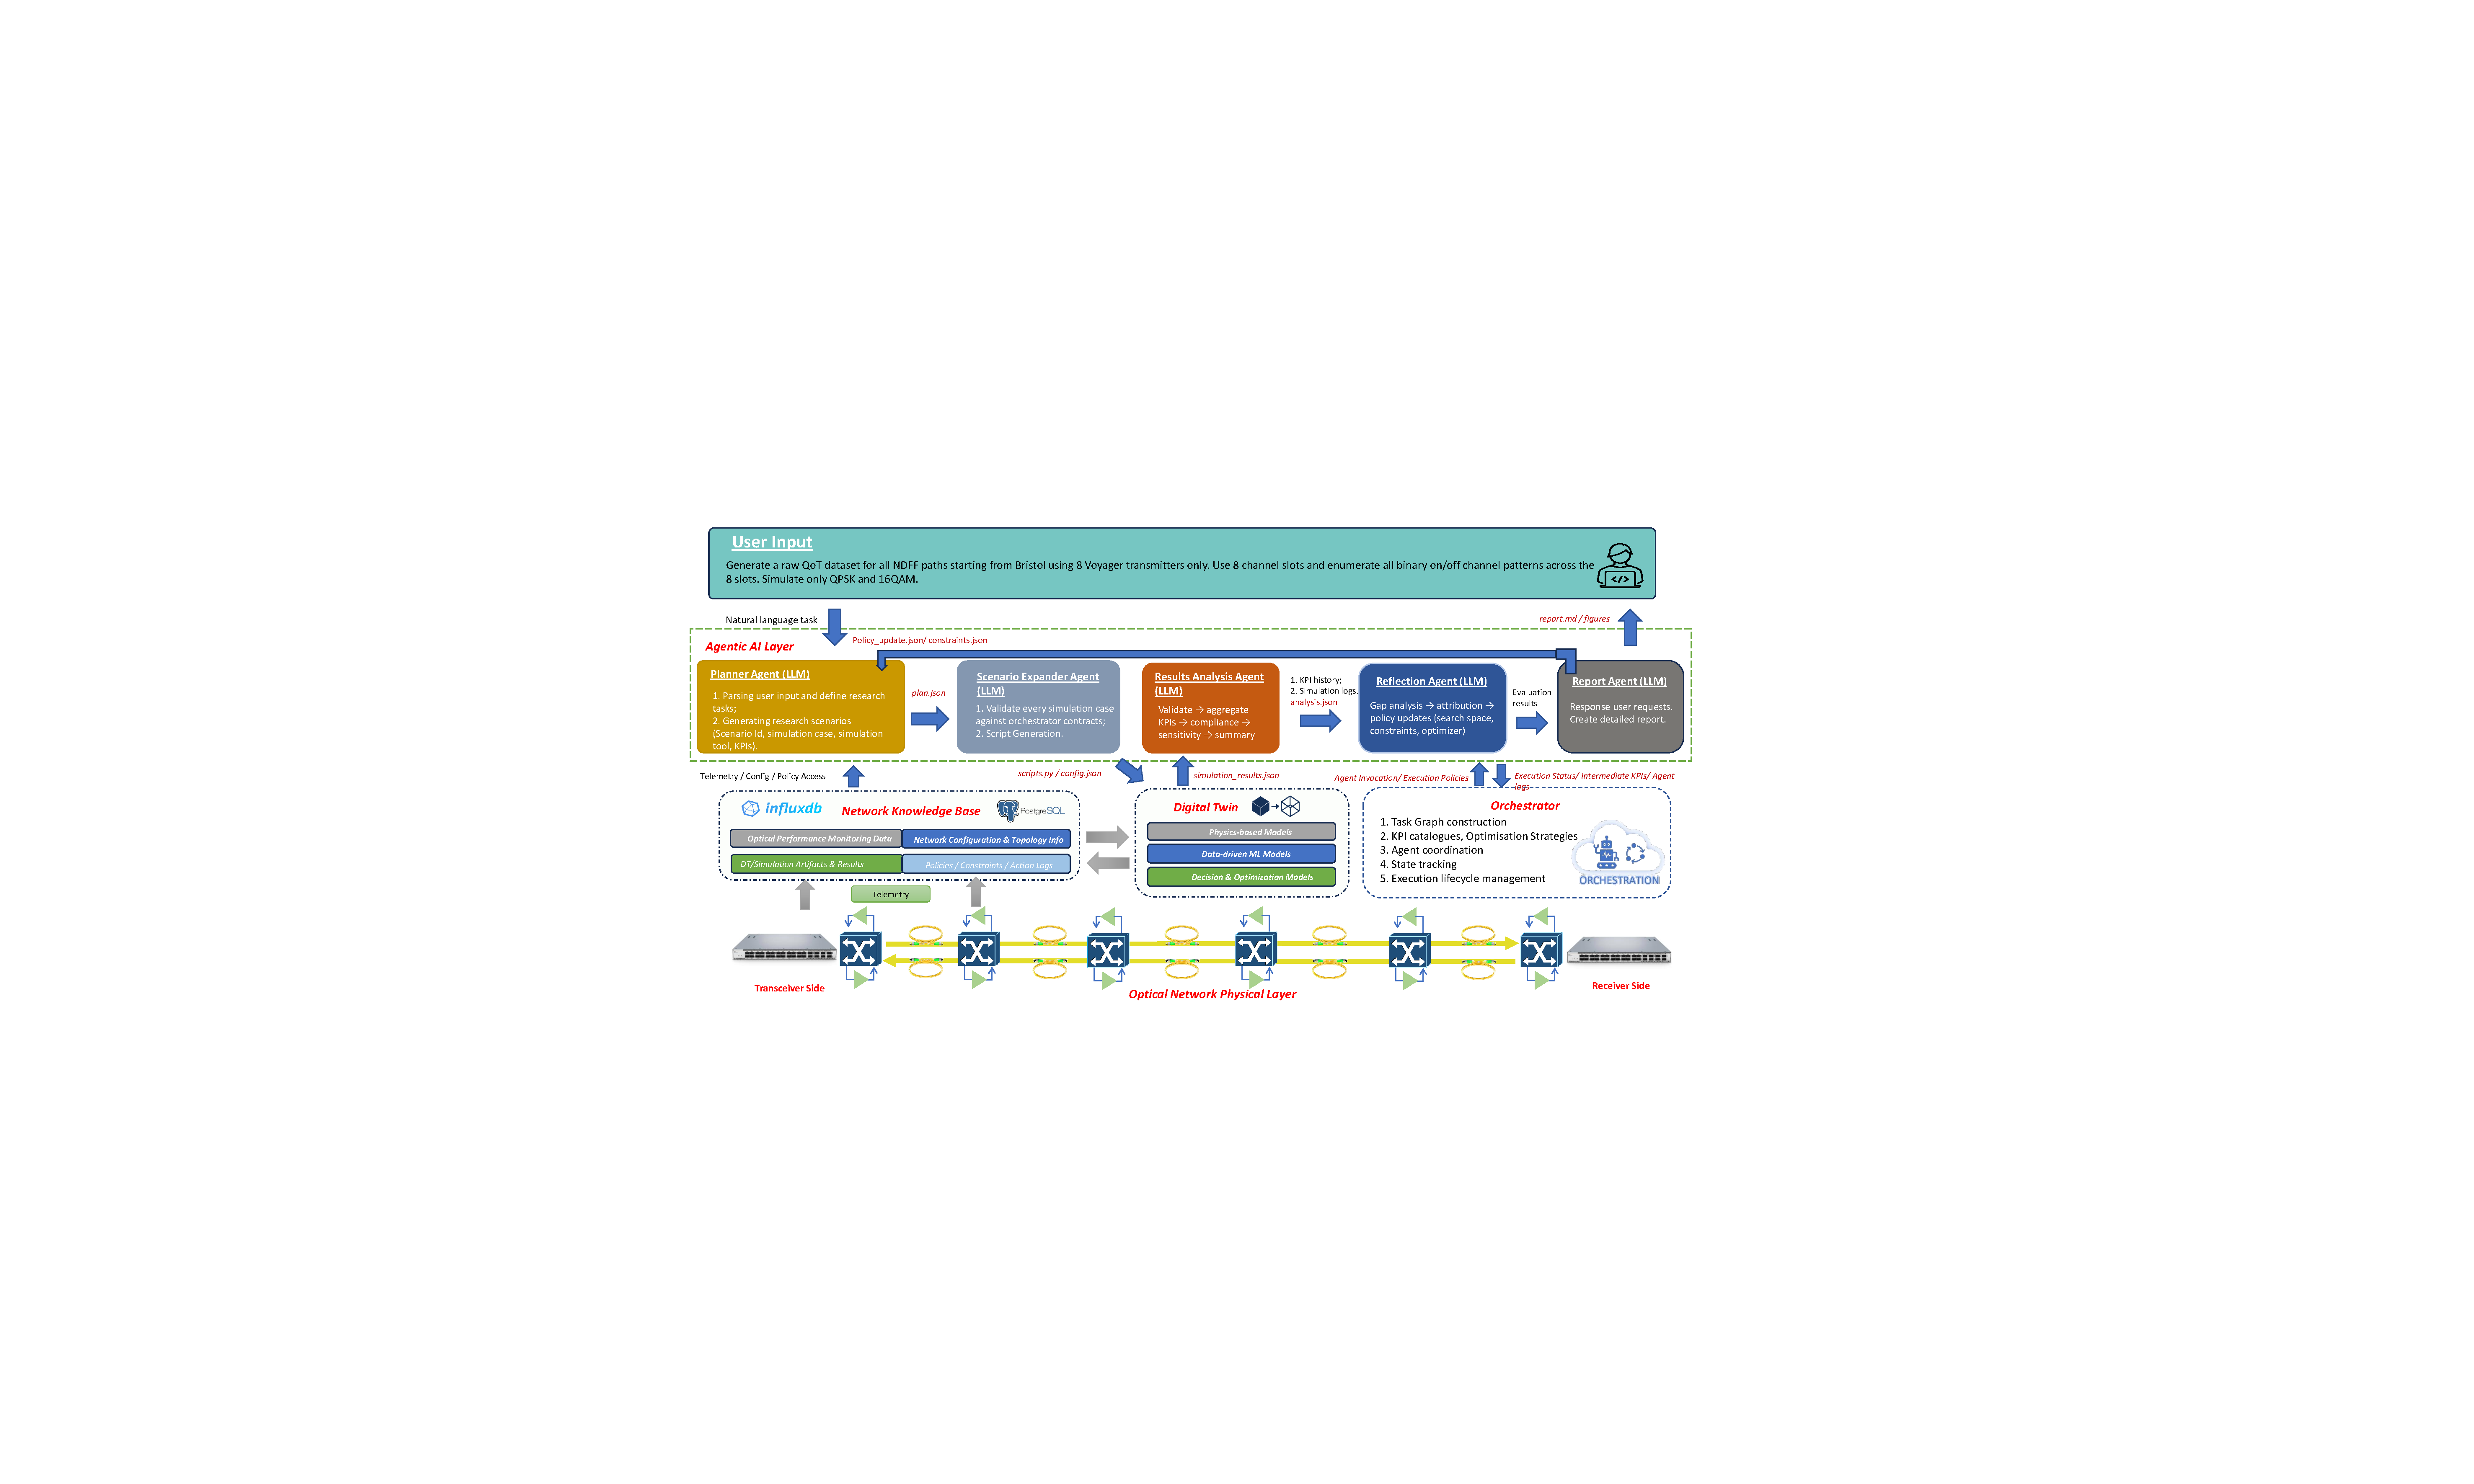
\includegraphics[width=\textwidth,pagebox=cropbox]{Figures/Architecture_Fig6.pdf}
    \captionsetup{justification=centering}
    \caption{Five-role data-generation architecture. Fig.~\ref{fig:proposed architecture.png} provides the framework scope, whereas this figure shows the role sequence, shared task state, simulator interface, and retained artefacts.}
    \label{fig:architecture_LLM}
    \vspace{-0.3cm}
\end{figure*}

\section{LLM-Driven Multi-Agent Digital Twins for Automated Cross-Domain Data Generation}
\label{sec:LLM}

Practical telemetry cannot cover every topology, loading condition, or rare event. This section evaluates an LLM-driven multi-agent DT workflow for generating complementary synthetic data.



\subsection{Proposed LLM-Driven Multi-Agent Digital Twin Framework}

Figure~\ref{fig:architecture_LLM} presents a five-role LLM-driven architecture coordinated through orchestrator-owned shared state. In the feasibility run reported below, Planner, Scenario Expansion, and Reflection invoked the LLM, while Results Analysis and Report used deterministic code for KPI aggregation and artefact packaging. Topology and equipment files, KPI definitions, simulator wrappers, and stored execution results provide the roles' knowledge and tools. The orchestrator passes a natural-language request through planning, scenario expansion, DT execution, analysis, optional refinement, and reporting. Role-specific input/output schemas preserve intermediate artefacts and allow individual roles to be inspected or replaced by deterministic functions.

The workflow invokes GNPy and ns-3 as DT engines and retains structured requests, configurations, results, and logs. Planner converts the user request into a study specification, Scenario Expansion produces simulator-ready cases, Results Analysis computes KPI summaries, Reflection proposes a revised parameter sweep, and Report packages the retained artefacts. This division makes the role sequence auditable; the deterministic baseline below provides the reference for the fixed configuration-enumeration task.

\subsection{Evaluation Protocol and Reproducibility}

We compare the GNPy demonstration with an independent deterministic enumerator over four destinations, two modulation/slot-width settings, 256 occupancy patterns, and three launch powers. Configuration keys exclude iteration and scenario identifiers, allowing repeated executions to be separated from the 6,144 unique cases. The script provides a configuration-set reference by enumerating the Cartesian product; intent parsing and optical propagation remain part of the orchestrated simulator workflow.

For reproducibility, a separately labelled instrumented run used \texttt{gpt-4o-mini-2024-07-18}, temperature 0.2, a 90-s timeout, at most three attempts per call, and strict mode. Planner, Scenario Expansion, and Reflection were each called twice. All six API calls succeeded on their first attempt, using 108,308 tokens, 26.22~s summed API latency, and an estimated \$0.01727 in text-token cost. Complete prompts, responses, logs, recovery history, and source/input hashes are available in the revision repository~\cite{JOCN_revision_code_2026}. The trace also records manual recovery during simulator execution, so the reported measurements characterise one fully documented workflow run.


\begin{table}[t]
\caption{Instrumented LLM workflow run.}
\label{tab:llm_trace}
\centering
\small
\setlength{\tabcolsep}{4pt}
\begin{tabularx}{\columnwidth}{p{2.15cm}X}
\hline
Item & Observed value \\
\hline
Model/settings & \texttt{gpt-4o-mini-2024-07-18}; temperature 0.2; timeout 90~s; maximum three attempts; strict mode \\
Role calls & Planner 2; Scenario Expansion 2; Reflection 2 \\
API outcomes & 6/6 successful first attempts; 0 retries; 0 API failures \\
Token usage & 106,041 prompt; 2,267 completion; 108,308 total \\
API latency & 26.22~s summed; 2.88--7.61~s per call \\
Estimated cost & \$0.01727 using the execution-date pricing snapshot \\
Retained evidence & Rendered requests/responses, call log, recovery record, and source/input hashes \\
\hline
\end{tabularx}
\end{table}

\begin{table}[t]
\caption{Configuration-set baseline for the GNPy demonstration.}
\label{tab:llm_baseline}
\centering
\small
\setlength{\tabcolsep}{4pt}
\begin{tabular}{lrrr}
\hline
Method & Executions & Unique & Duplicate rate \\
\hline
Deterministic enumerator & 0 & 6,144 & 0 \\
LLM-orchestrated history & 8,192 & 6,144 & 25\% \\
\hline
\end{tabular}
\vspace{2pt}

\footnotesize Both sets have precision and recall 1.0 against the independently specified 6,144-key set. The deterministic baseline uses no LLM/API calls and provides a configuration-set reference; its execution count excludes simulator runs.
\end{table}

\subsection{Use Cases and Demonstration Results}

We demonstrate the workflow with GNPy for optical transport and ns-3 for wireless access. The generated data, simulator source, and supporting validation artefacts are available in the cited repositories~\cite{Shen_dataset_2026,JOCN_revision_code_2026}.


\begin{figure*}[t]
    \centering
    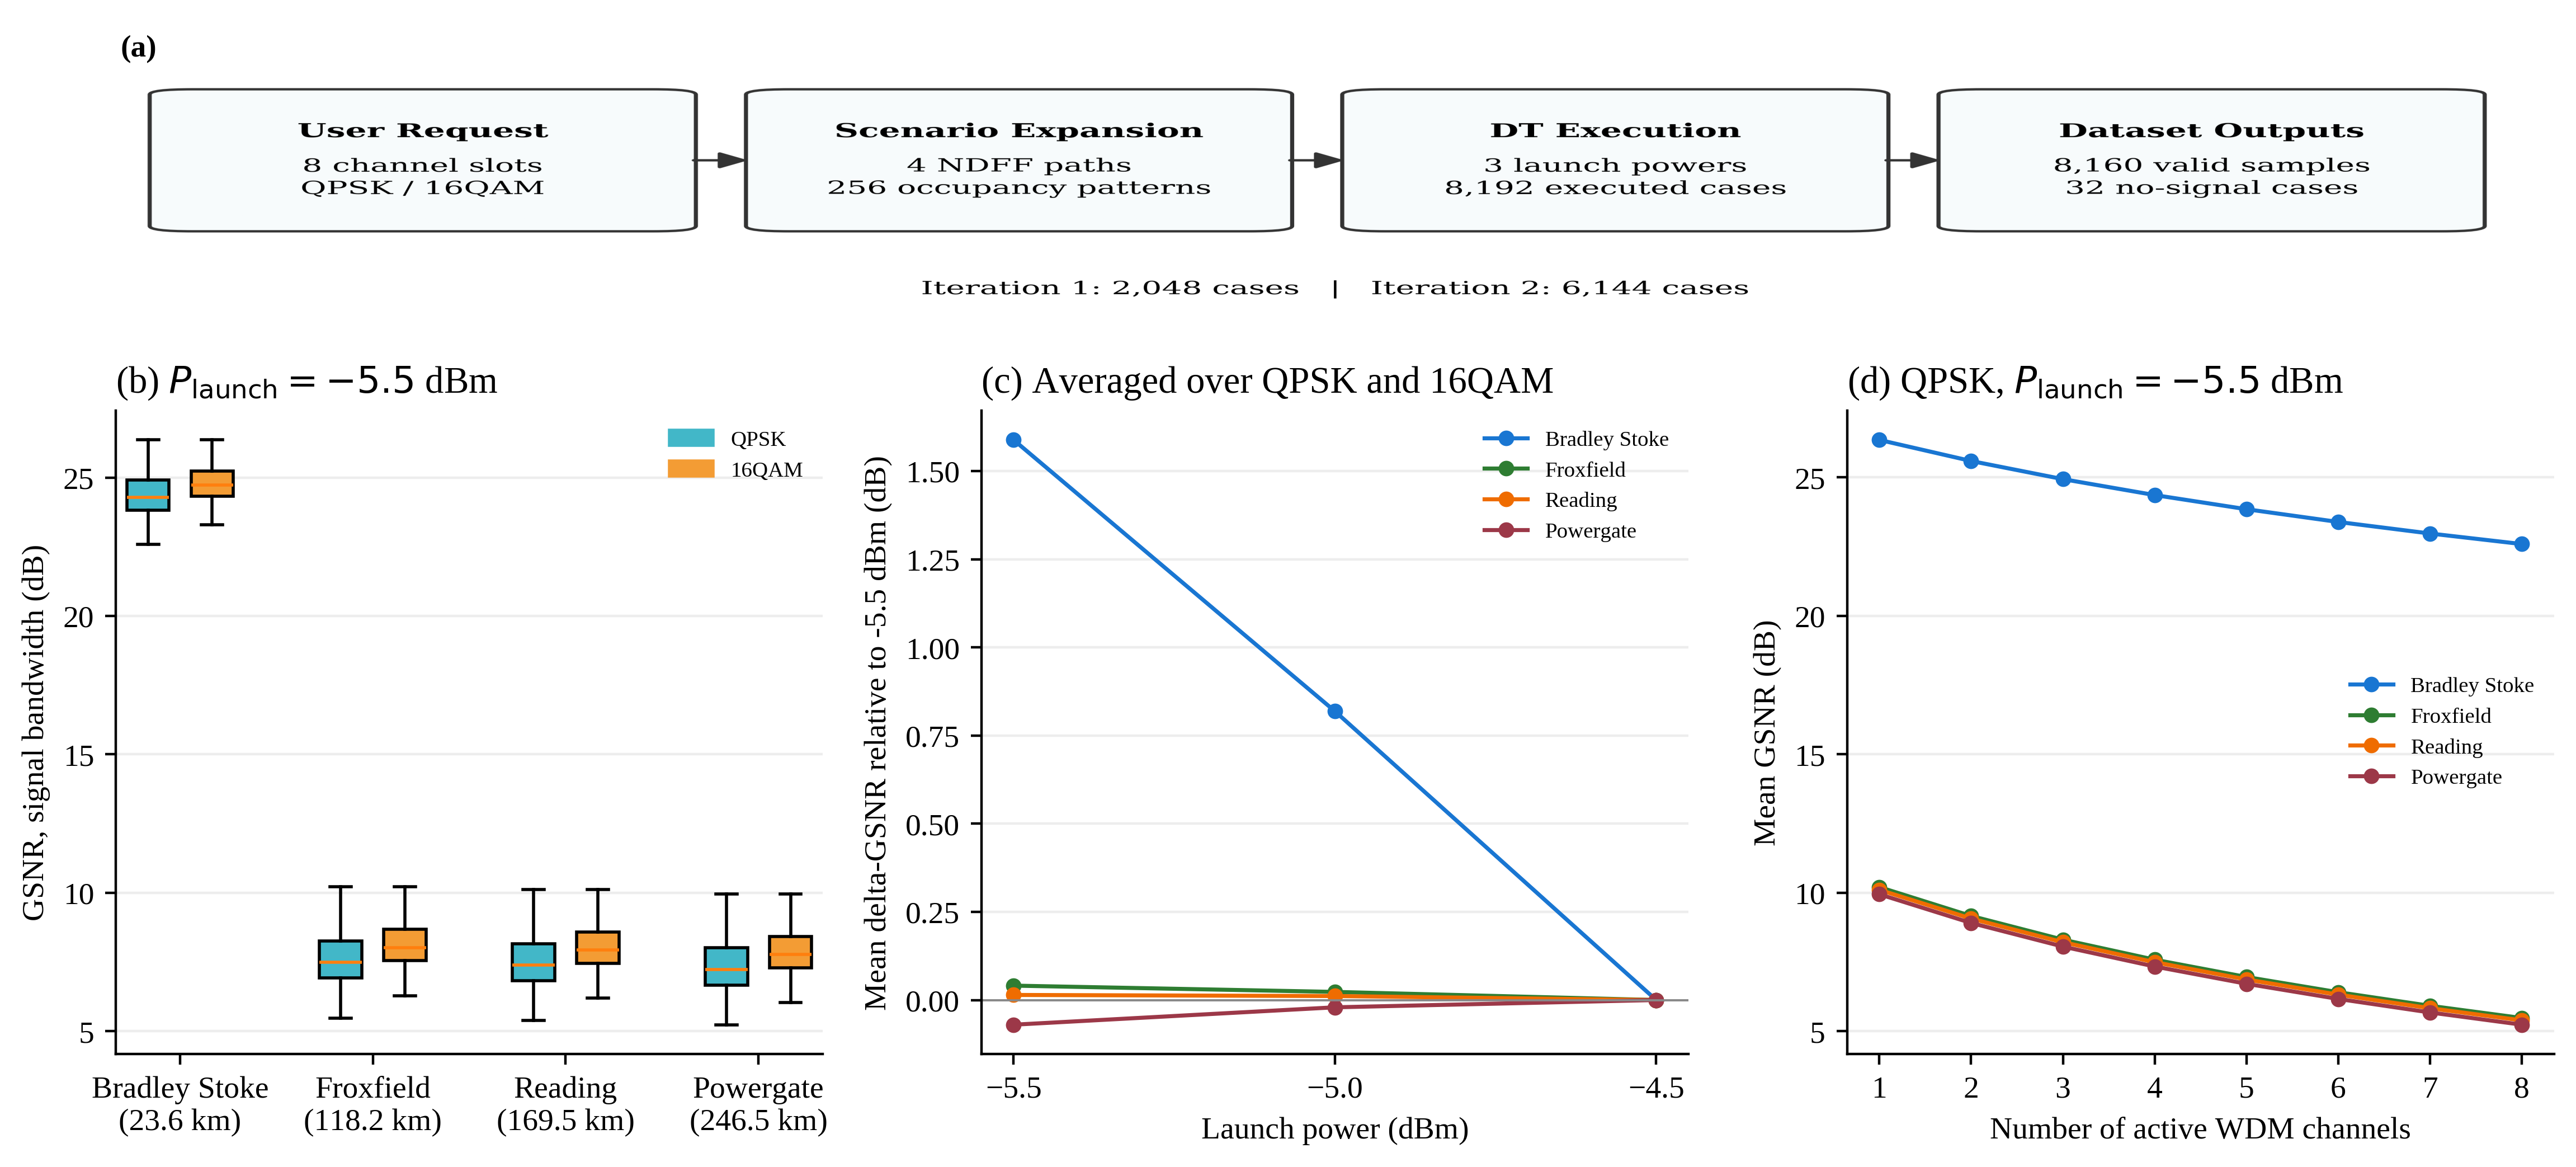
\includegraphics[width=0.98\linewidth]{Figures/usecase1_highres.png}
    \captionsetup{justification=centering}
    \caption{GNPy-based optical QoT dataset generation over the NDFF topology. (a) Agent-driven scenario expansion and dataset-generation workflow, (b) GSNR distributions for QPSK and 16QAM over the four paths at $P_{\mathrm{launch}}=-5.5$~dBm, (c) route-dependent GSNR variation with launch power, averaged over QPSK and 16QAM and normalised to the results at $-5.5$~dBm, (d) mean GSNR as a function of the number of active WDM channels for QPSK transmission at $P_{\mathrm{launch}}=-5.5$~dBm.}
    \label{fig:usecase1}
    \vspace{-0.3cm}
\end{figure*}

\subsubsection{GNPy-Based Network-Level QoT Data Generation}

In this use case, the proposed LLM-driven multi-agent DT framework generates an optical QoT dataset over the NDFF topology. The request considers four paths originating from Bristol, Voyager transmitters, eight WDM channel slots, and QPSK and 16QAM configurations. The Planner Agent defines the study scope and target KPIs, while the Scenario Expansion Agent constructs the optical paths, binary channel-occupancy patterns, and launch-power settings for GNPy execution.

As illustrated in Fig.~\ref{fig:usecase1}(a), the four paths, two modulation/spectrum configurations, and $2^8=256$ occupancy patterns produce 2,048 cases per launch power. The archived workflow first evaluates $-5.5$~dBm and then executes a refined sweep at $-5.5$, $-5.0$, and $-4.5$~dBm. Across the two passes, it produces 8,192 execution records, of which 8,160 contain numerical QoT results and 32 correspond to all-off channel states with no optical signal.

Figure~\ref{fig:usecase1}(b)--(d) shows route-, launch-power-, and channel-loading-dependent GSNR variation. Over the tested launch-power range, the Bristol--Bradley Stoke path decreases by approximately 1.59~dB, whereas the longer paths show smaller changes. At $-5.5$~dBm, the mean QPSK GSNR decreases from 26.35 to 22.59~dB on the Bristol--Bradley Stoke path and from 9.95 to 5.24~dB on the Bristol--Powergate path as the number of active channels increases from one to eight. Independent replay supports numerical reproducibility under the pinned GNPy environment, while also indicating sensitivity to simulator version. The complete configurations and reproducibility artefacts are provided in the released repository~\cite{Shen_dataset_2026}.


\subsubsection{ns-3-Based Multi-Access Network Performance Data Generation}
\label{sec:ns3_wireless}

In this use case, the proposed LLM-driven multi-agent DT framework assists in the automatic construction of ns-3 scenarios for synthetic wireless dataset generation. The aim is to convert a high-level request into an executable indoor scenario with three mobile CPEs and three access branches: Wi-Fi 802.11n, an LTE/EPC cellular branch, and a LiFi-like access link. The target KPIs are per-flow throughput, FlowMonitor-reported packet loss, mean delay, and mean jitter over a 10-s simulation.

The Planner Agent formulates the task, and the Scenario Expansion Agent produces the simulator configuration and executable source. Each CPE is a multi-homed node with one interface per branch and a common mobility state. The cellular branch uses ns-3 LTE/EPC helpers, the Wi-Fi branch uses the native 802.11n model, and the LiFi-like branch is implemented as a CSMA-based LiFi surrogate with a configurable link rate for packet-level multi-access evaluation. The implementation, configuration, and generated data are provided in the released workflow repository~\cite{JOCN_revision_code_2026}.

\begin{figure*}[t]
    \centering
    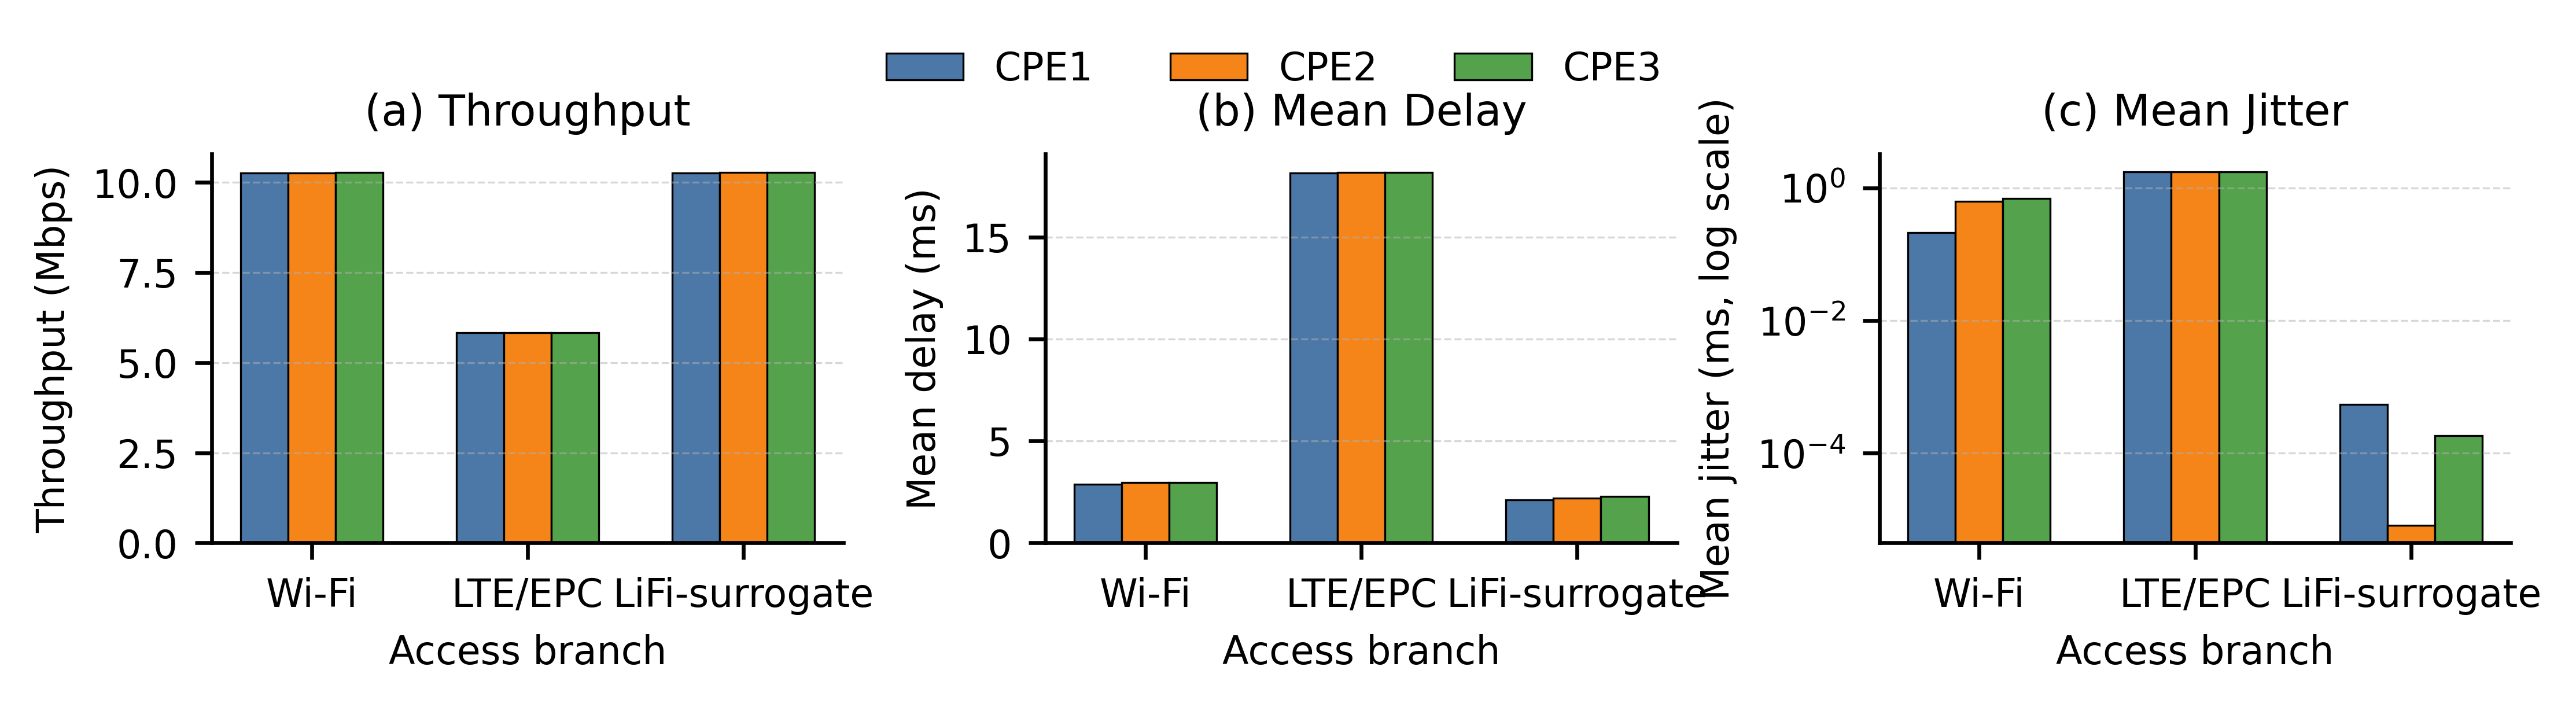
\includegraphics[width=0.98\linewidth]{Figures/fig_ns3_results.png}
    \captionsetup{justification=centering}
    \caption{FlowMonitor-derived per-flow KPIs for one representative ns-3 configuration (10~Mbps per flow, 3~m/s, 100-Mbps LiFi-surrogate rate, seed 2): (a) throughput, (b) mean delay, and (c) mean jitter across Wi-Fi 802.11n, LTE/EPC, and the CSMA-based LiFi surrogate. The results are specific to the stated simulation configuration.}
    \label{fig:ns3_results}
    \vspace{-0.3cm}
\end{figure*}

The bounded sweep combines four offered loads (2, 5, 10, and 20~Mbps), two mobility speeds (0.5 and 3~m/s), two LiFi-surrogate rates (50 and 100~Mbps), and three seeds, giving 48 configurations. Each configuration produces three application flows per branch, yielding 432 application-flow records; the 624 raw FlowMonitor rows additionally include infrastructure flows. Packet loss denotes the FlowMonitor-reported ratio rather than terminal loss, because packets may remain in flight when the 10-s simulation ends.

Correctness was evaluated independently of the original KPI exporter. FlowMonitor XML was re-parsed for all 48 runs, and all application-flow packet counters matched exactly; the maximum reconstruction differences were $5.57\times10^{-5}$~Mbps for throughput, $3.16\times10^{-3}$~ms for delay, and $1.10\times10^{-5}$~ms for jitter, attributable to XML time serialisation. Three representative configurations were rebuilt and replayed with zero KPI delta, a fixed-seed configuration produced identical results in two executions, and a separately written ns-3 reference passed five topology/configuration checks and all 63 KPI comparisons~\cite{Shen_dataset_2026}.

Figure~\ref{fig:ns3_results} shows access-dependent KPI patterns under the representative configuration. In particular, the very small LiFi-surrogate jitter reflects the idealised CSMA implementation. Overall, the use case demonstrates automated ns-3 scenario construction, execution, KPI extraction, and bounded reproducibility under the declared models. The resulting synthetic dataset is separate from the measured 5G NR, Wi-Fi~6, and LiFi testbed data, and the reported KPI differences are interpreted within the stated simulation configuration.

\section{Conclusions}
We presented an openly available cross-domain dataset framework for optical transport, fibre sensing, and wireless access, combining practical telemetry, semantic abstraction, and synthetic DT-generated data. Cross-domain is realised by the system architecture and unified data interfaces. Although experimental-platform scheduling required the practical datasets to be collected in different time periods, the training workflow invokes domain-specific preprocessing and accesses optical and wireless features through a common interface.

On the semantic-fusion benchmark, the three-dimensional semantic representation preserves the binary-task utility of the hand-crafted representation while moderately reducing observed CPE-attribute leakage, yielding an empirical privacy--utility trade-off. The LLM-driven multi-agent DT workflow provides auditable interaction with GNPy and ns-3; the deterministic baseline reproduces the fixed optical configuration set, and the LLM roles add intent interpretation and reflection-guided refinement. Versioned replay quantifies numerical reproducibility and simulator sensitivity. Future work will focus on calibrated physical models, expanded optical--wireless datasets, and repeated workflow evaluation on larger scenario spaces.

\section*{Acknowledgement}
This work was partly supported by the European Commission's Horizon research and innovation programme: Allegro project (No. 101092766) and the EU-funded project ECO-eNET (No. 10113933).

\bibliography{sample.bib}

\end{document}
